\documentclass[10pt,twocolumn,letterpaper]{article}

\usepackage{cvpr}
\usepackage{times}
\usepackage{epsfig}
\usepackage{graphicx}
\usepackage{amsmath}
\usepackage{amssymb}
\usepackage{makecell}

% Include other packages here, before hyperref.

% If you comment hyperref and then uncomment it, you should delete
% egpaper.aux before re-running latex.  (Or just hit 'q' on the first latex
% run, let it finish, and you should be clear).
\usepackage[breaklinks=true,bookmarks=false]{hyperref}

\cvprfinalcopy % *** Uncomment this line for the final submission

\def\cvprPaperID{****} % *** Enter the CVPR Paper ID here
\def\httilde{\mbox{\tt\raisebox{-.5ex}{\symbol{126}}}}

% Pages are numbered in submission mode, and unnumbered in camera-ready
%\ifcvprfinal\pagestyle{empty}\fi
\setcounter{page}{4321}
\begin{document}

%%%%%%%%% TITLE
\title{Text2Scene: Generating Compositional Scenes from Textual Descriptions}

\author{Parm Johal\\
{\tt\small parmj@uvic.cag}
\and
Sean McFarlane\\
{\tt\small seanmcf@uvic.ca}\\
University of Victoria\\
3800 Finnerty Road, Victoria, BC
\and
Simon Walker\\
{\tt\small walker11@uvic.ca}
}

\maketitle
%\thispagestyle{empty}

%%%%%%%%% ABSTRACT
\begin{abstract}
In this paper, we extend the proposal of Text2Scene, a model generating different types of compositional scene representations using natural language descriptions. In this extended experimentation, we start off by using long short-term memory (LSTM) instead of gated recurrent units (GRU) for image encoding. We focus our experimentation on an altered version of the abstract scenes dataset to exhibit the similarities and differences in accuracy and computation between the two networks. We then proceed to combine the LSTM recurrent units with a different network architecture, called ResNeXt, in place of the ResNet architecture used in the original experiments. After combining these 3 alterations, we are able to obtain competitively accurate results when compared to the original model.
\end{abstract}

%%%%%%%%% BODY TEXT
\section{Introduction}
Our project takes the original Text2Scene model and enhances some parts that have been outdated due to recent discoveries. After receiving the original code, running it took hours to compute a few epochs. We decided that the first improvement to make would be to speed up the execution of the network. Motivated by this, we decided to use a new architecture called ResNeXt which would increase the speed at which each epoch processes the data (figure \ref{runtime}). We further worked on implementing our own data set by replacing objects in the scene (table \ref{objectrep}) and setting up TensorBoard to allow us to monitor accuracy and loss. Due to problems on the user side we were not able to fully implement the TensorBoard.\par
Images are encoded in the original Text2Scene by using gated recurrent units (GRU) and long short-term memory (LSTM). GRU is a gating mechanism in recurrent neural networks used to solve the vanishing gradient problem, which is when the gradient eventually becomes insignificant and prevents the weight from changing its value. The LSTM is a better version of a GRU since it can be used with bigger datasets because of its modified gates based off of the ones in the GRU. From this, we hypothesize that the dataset we are using will work better if we encode the data using the LSTM rather than the GRU considering the amount of data that is being processed.\par
With these changes we are able to describe and show the improvements we contribute to the Text2Scene model. In the following sections we will discuss some related work, the original and updated model, our experiments and improvements, and finally our conclusion.
Our contributions are summarized as follows:
\begin{itemize}
 \item We show that by changing to the ResNeXt architecture we can increase the accuracy and runtime of the model.
 \item We generate a modified dataset to conduct experiments on.
\end{itemize}


\section{Related Work}
In the original project made by Tan et al.\cite{1}, they noted other related works on this topic such as generated captions from images \cite{4, 5} and text-to-image synthesis \cite{6, 7}. What they noticed was that even though these works gave quality information from their experiments, they were not taking into account scenes in which multiple objects interact with each other. This was why they proposed their Text2Scene model which “produces a scene by sequentially generating objects (e.g. in the forms of slip-arts, bounding boxes, or segmented object patches) containing the semantic elements that compose the scene” \cite{1}. \par
Some works that were closely related to the original Text2Scene are \cite{8, 9, 10}. Johnson et al \cite{8} used structured scene graphs to generate their images by having the objects and their details be the inputs to the graph. In Text2Scene the objects effect on the overall image (placement, orientation, etc.) is inferred from text. Hong et al \cite{9} generated layouts as representations in a trained module unlike the work from before. Due to this their results were not as accurate as Text2Scene since they generated pixel-level outputs which gave a stronger result which is seen in the overall image. Gupta et al \cite{10} generated cartoon-like images by having the presented objects be the input to the model, and the predictions of how the scene will be generated were done by separably trained modules. Text2Scene instead does more realistic scenes and uses an “end-to-end”\cite{1} way of training. To Tan et al \cite{1}, the Text2Scene model was one of the first to go beyond cartoon-like imagery and be capable of generating detailed scenes under a single working framework.

\section{Model}
\subsection{Dataset}
The original dataset was constructed by using turkers to generate 10,020 variations of an original 1002 manually constructed seed scenes, with 10 variations on each original scene. The result of the turking was 10,020 scene layouts stored as object coordinates in Scenes\_10020.txt. The data in Scenes\_10020.txt was then fed into SceneRenderer.exe, which composes each final scene image out of individual source object images based on the coordinates given. Additional metadata is constructed that is used by the network to form associations. An object list is created, which identifies certain words as entities in the scene. A relation list enumerates different ways scene objects are paired together. A bag-of-words representation for each description is created along with a list of all words sorted by their frequency. The resultant 10,020 scene images and 10,020 scene descriptions are fed into Text2Scene as input, along with the metadata, and used to train the model.
\subsection{Image Encoding}

\begin{figure}[t]
\begin{center}
    \fbox{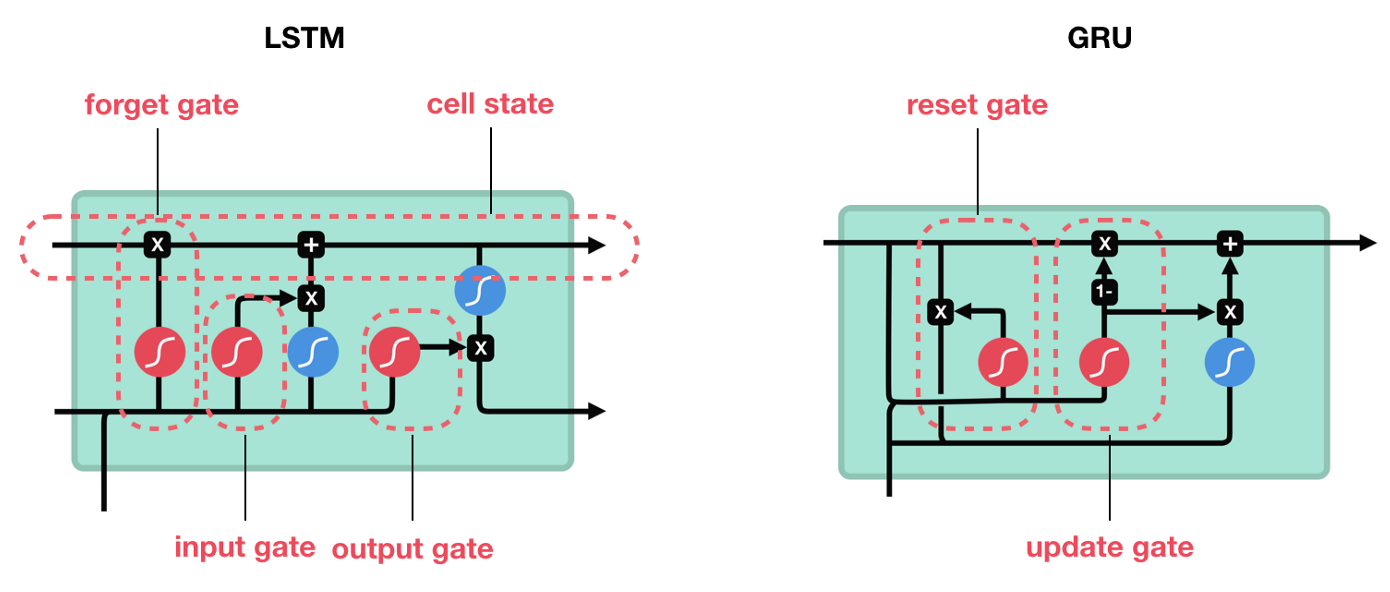
\includegraphics[width=0.8\linewidth]{lstmvgru.png}}
\end{center}
   \caption{Gate structure comparison between LSTM and GRU.\cite{3}}
\label{lstmvgru}
\end{figure}

In this model we use LSTM to resolve short term memory in the RNN. LSTM is used instead of GRU since it uses more training parameters and it is more accurate with datasets involving longer sequences of data \cite{3}. This is shown in figure \ref{lstmvgru}, as LSTM is shown having more gates. This leads to better control of the output and hence, better accuracy. Since the original model learns to sequentially generate objects and their attributes at each time step \cite{1},  we use LSTM to aid this task.

\subsection{Pre Trained Network Architecture}

\begin{figure}[t]
\begin{center}
   \fbox{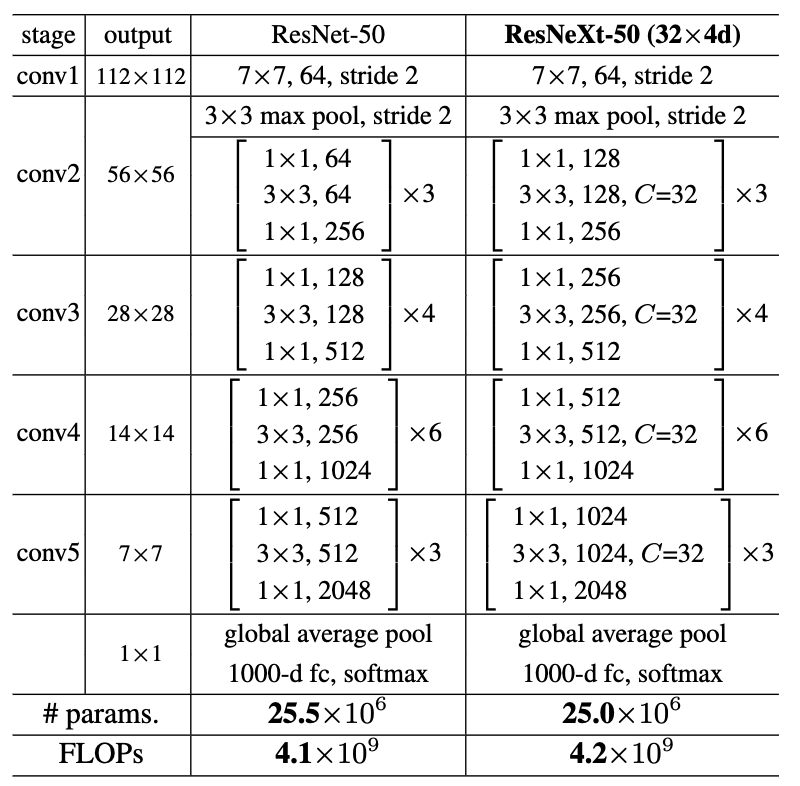
\includegraphics[width=0.8\linewidth]{resnext.png}}
\end{center}
   \caption{Resnet vs. ResneXt \cite{1}}
\label{resnext}
\end{figure}


The pretrained network consists of a highly modularized version of the currently established ResNet architecture. The network is developed by repeating a building block that sums a set of transformations with the same topology \cite{12}, which is shown in figure \ref{resnext}. Unlike the original ResNet architecture, the ResNeXt architecture keeps track of the number of paths it goes through, using ‘C’ as the variable above.


\section{Experiments}

Since time constraints were a significant issue, tests were limited to between 1 and 5 epochs. Tests were performed on the original dataset and model, the altered dataset with LSTM, the original dataset with ResNeXt and LSTM,  and the altered dataset with ResNeXt and LSTM.

\subsection{Changing Architecture}
\begin{figure}[t]
\begin{center}
   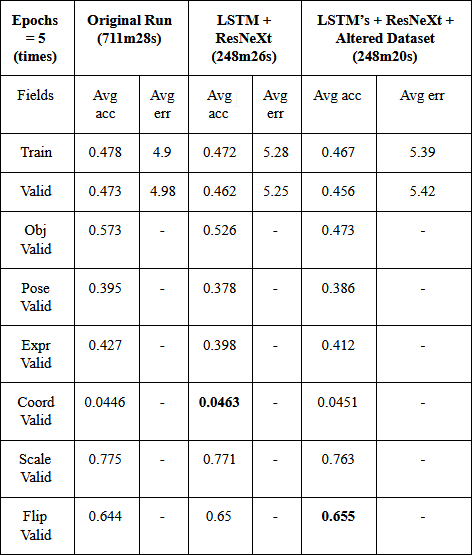
\includegraphics[width=0.8\linewidth]{archplot.png}
\end{center}
   \caption{Results after training the revised model.}
\label{archplot}
\end{figure}

After running the original model, we proceed to run the same model with the LSTM + ResNeXt architectural change. The results can be seen in figure \ref{archplot}. The move to a new architecture significantly improved the efficiency of the training, but at the cost of accuracy. The training accuracy dropped by 0.6\% and the validation accuracy by 1.1\%. However, we are able to see an increase in accuracy for the coordinate validation field by 0.17\%.

\subsection{Adding Altered Dataset}

Due to feasibility constraints an entirely new dataset could not be constructed. The original dataset makes extensive use of turking in its creation which puts it outside the scope of what we have available. As an alternative, the original scene layouts were used, but with certain objects replaced in every scene they appear. Additionally, any textual references to these objects are replaced. This would, at the very least, allow us to test the neural network on novel image and text data, and examine how it adapts with training. The modified scene objects are listed in table \ref{objectrep} .

\begin{table}
\begin{center}
\begin{tabular}{|c|c|}
\hline
Original Object & Replacement Object \\
\hline\hline
Baseball bat & Katana \\
Pirate hat & Top hat \\
Pie & Cake\\
Snake & Armadillo\\
Dog & Duck\\
\hline
\end{tabular}
\end{center}
\caption{Objects that were replaced in the modified dataset.}
\label{objectrep}
\end{table}

The original images were replaced with new PNG files, and text references to these objects were replaced in all the textual input data. The replacements were selected to still fit the contexts the originals were used in, since the layouts of the scenes must remain the same. A script was used to automatically replace all occurrences of these objects in the text with their new versions. Additionally, some other phrases in the 10,020 scene descriptions were replaced to match the new objects, some examples of which can be seen in table \ref{phrasereplace}.


\begin{table}
\begin{center}
\begin{tabular}{|c|c|c|}
\hline
Replaced object &\makecell{ Original \\reference} & \makecell{Replaced \\  reference}\\
\hline\hline\hline
Pirate hat & \makecell{...wants to be \\\textbf{a pirate}}. & \makecell{...wants to be\\ \textbf{dapper}}.\\
\hline
Baseball bat & \makecell{...is playing \\\textbf{baseball} in the...} & \makecell{...is playing \textbf{with}\\ \textbf{swords} in the...} \\
\hline
\end{tabular}
\end{center}
\caption{Phrases associated with the objects which were modified.}
\label{phrasereplace}
\end{table}

 After the original PNG files were replaced, the SceneRenderer executable included with the data was used, which generated 10,020 unique scenes composed from the new source images. An additional script was created to update the metadata such as the bag-of-words representation and occurrence-count word list, as no functionality to generate this data was included with the original dataset.

\begin{figure}[t]
\begin{center}
   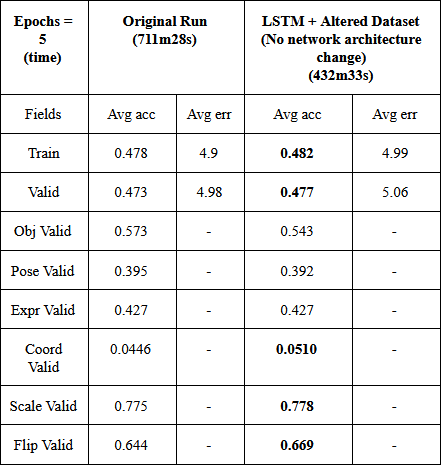
\includegraphics[width=0.8\linewidth]{dsetplot.png}
\end{center}
   \caption{Results from using only LSTM with the altered dataset.}
\label{dsetplot}
\end{figure}

\begin{figure}[t]
\begin{center}
  \fbox{
\includegraphics[width=0.8\linewidth]{sceneimg.png}}
\end{center}
   \caption{A generated scene using the new "Top Hat" and "Duck" objects.}
\label{sceneimg}
\end{figure}

\subsection{Results}

\begin{figure*}[t]
\begin{center}
  \fbox{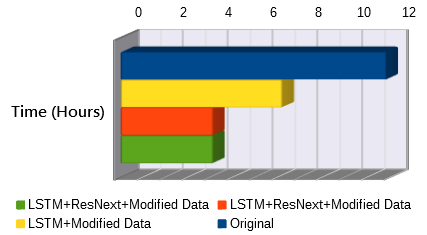
\includegraphics[width=0.6\linewidth]{runtime.png}}
\end{center}
   \caption{Total runtime over 5 epochs for each of the four tests.}
\label{runtime}
\end{figure*}

\begin{figure*}[h]
\begin{center}
  \fbox{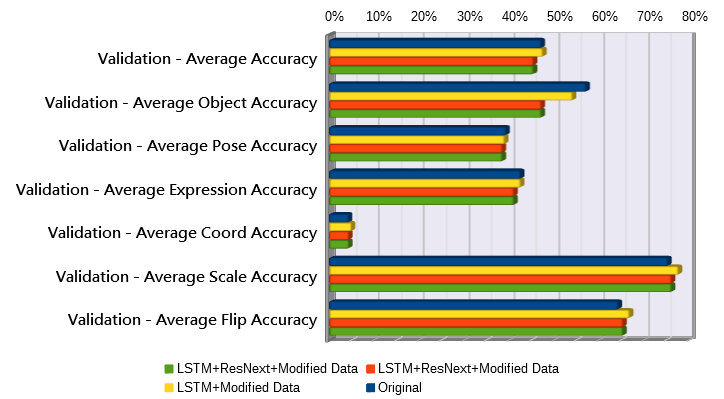
\includegraphics[width=\dimexpr\textwidth-2\fboxrule-2\fboxsep]{valstat.png}}
\end{center}
   \caption{Validation step scores for each of the tests conducted.}
\label{valstat}
\end{figure*}

Looking at the data between figures \ref{archplot} and \ref{dsetplot} we can see the results when the altered dataset is added. From figure \ref{archplot} we see a further decrease in training and validation accuracy (with the exception of the flip validation accuracy), but when the ResNeXt network architecture is replaced with the original ResNet network and used with the altered dataset we see a big improvement. More importantly, we see that the training and validation accuracies both improve by 0.4\%. This was an unexpected result as we anticipated an improvement on the dataset with ResNeXt, but instead we discovered better scores using ResNet.


\section{Conclusion}

Our changes to the original design of Text2Scene have increased the speed and accuracy of the training while retaining the specifics of the original work. Although we initially hypothesized the switch to ResNeXt giving us an increase in accuracy for our altered dataset, the ResNet implementation combined with LSTM surprised us with the increase in accuracy. The ResNeXt architecture  alongside the change of the dataset, however,  made it so that we can run the model in better time due to feasibility constraints. This improved runtime may even result in increased accuracy if given the same amount of time to train.

%
%
%
%
% END OF ACTUAL PROJECT CONTENT
%
%
%
%



%-------------------------------------------------------------------------
\newpage
\newpage
{\small
\bibliographystyle{ieee}
\bibliography{egbib}
}

\end{document}
